 \chapter{Experimental Tasks}

\begin{figure}[ht]
\centering
\includegraphics[width=.6\columnwidth]{Grafiken/measurement1.pdf}%
\caption{}%
\label{fig:measurement1}%
\end{figure}


\section{Recording of the U/I-Curve}

\begin{figure}%
\centering
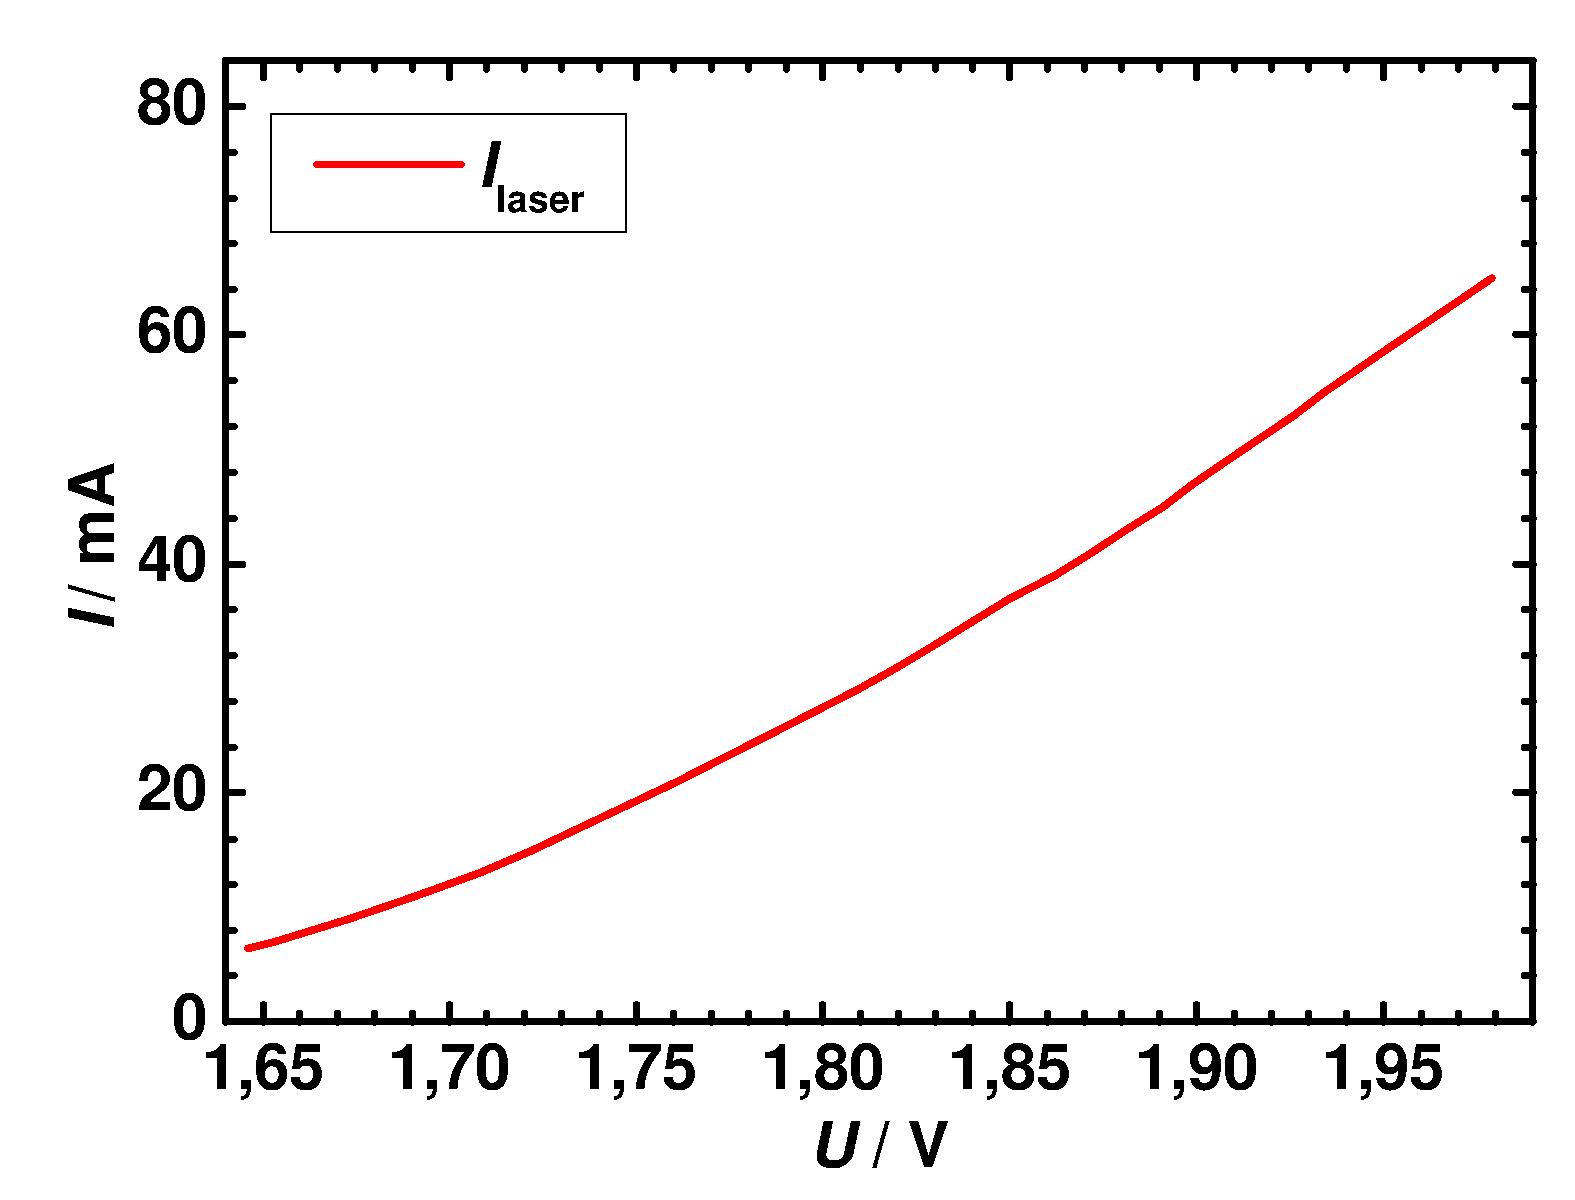
\includegraphics[width=.5\columnwidth]{Grafiken/1_IU.pdf}%
\caption{measured I/U curve at $T$~=~20~�C}%
\label{fig:1_IU}%
\end{figure}

 In the first experimental task the U/I-curve of the laser diode is recorded. This is done by biasing the diode with a current and measuring the voltage (cf. Figure \ref{fig:measurement1}a). The bias current is increased from a minimum of 6.4~mA to 65~mA in steps of 2~mA. The resulting $U/I$-curve is shown in Figure \ref{fig:1_IU}.

From
\begin{equation}
 \begin{split}
I = I\i{S0}\left[\e^{\beta\left(U-R\i{s}I\right)}-1\right] \hspace{2cm} I\leq I\i{S}\\
U = W\i{G}/e +R\i{S}I \hspace{2cm} I\geq I\i{S}\\
 \end{split}
\end{equation}
follows for the current above threshold:
\begin{equation}
 I = \frac{W\i{G}/e}{R\i{S}}-\frac{U}{R\i{S}}% = a + b\cdot U
 \label{eq:I/U}
\end{equation}
%The coefficients a and b can be determined by fitting a linear function to the U/I-curve above the threshold. The threshold current is calculated later in section \ref{ch:threshold}.  With these coefficients the band gap and the serial resistance of the laser diode can be calculated as:
\comwo{Mir ist nicht klar, wof�r du den linearen Fit brauchst. Ich habe das jetzt mal auskommentiert. Ich habe einfach in die �ber dem kommentar stehende Formel zwei messwerte weit oberhalb der Threshold-Spannung eingesetzt und damit dann zwei gleichungen aufgestellt}

Inserting two values of the linear range above threshold ($U(65~\mathrm{mA})=1.979~\mathrm{V}$ and $U(59~\mathrm{mA})=1.952~\mathrm{V}$) into \eqref{eq:I/U} leads to two equation which can be solved for $W\i{G}$ and $R\i{S}$:
\begin{equation}
\begin{split}
 W\i{G}=1.6865~\mathrm{eV}\\
 R\i{S} = 4.5~\Omega
\end{split}
\end{equation}
The bandgap of 1.6 corresponds to a wavelength of $\lambda =~$736~nm using 
Using 
\begin{equation}
W\i{G}=\frac{hc}{\lambda\i{G}}
\label{eq:}
\end{equation}
the to the bandgap corresponding wavelength can be calculated: 
\begin{equation}
\lambda\i{G}=736~\mathrm{nm}\quad.
\label{eq:}
\end{equation}


\section{P/I-Curve}
The output power of the laser diode at different driving currents is measured with a reference detector at the rear mirror of the laser resonator. Because the reflectivity is the same at both mirrors of the laser diode, the measured power is identical with the power emmitted in the other direction. The setup for measuring is shown in figure \ref{fig:measurement1}b.
\begin{figure}%
\centering
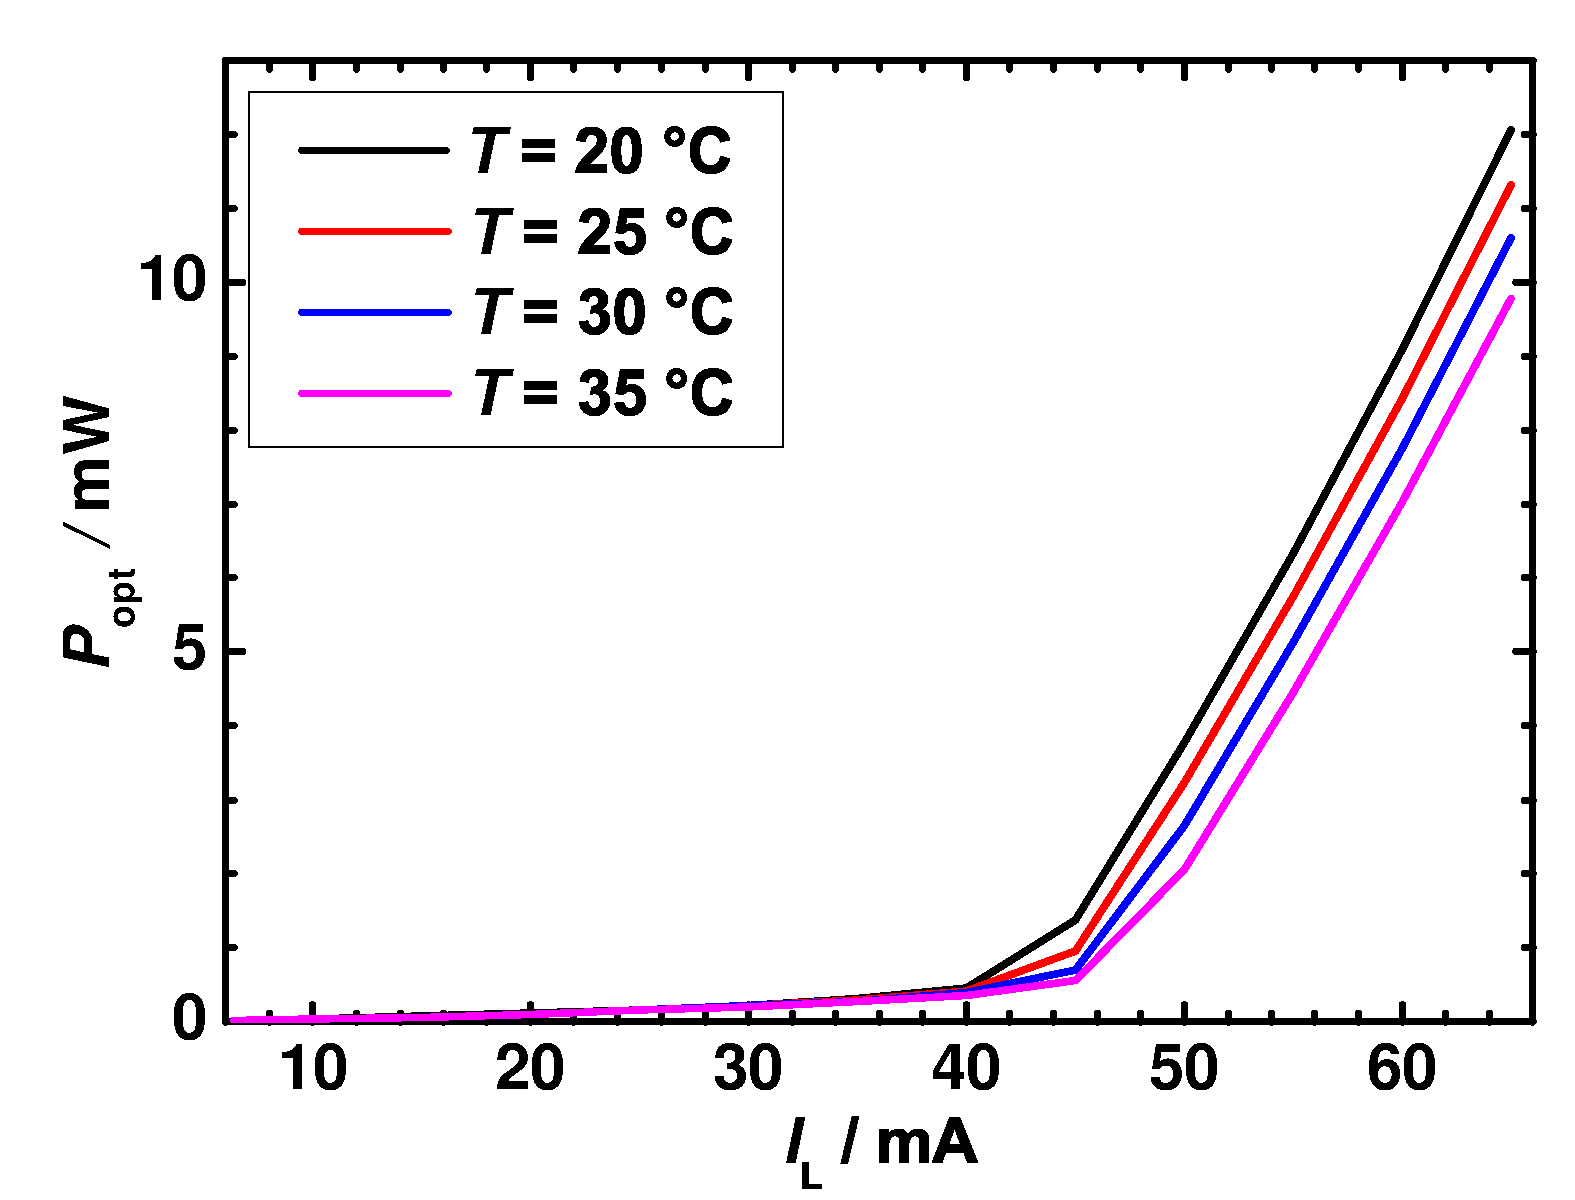
\includegraphics[width=.5\columnwidth]{Grafiken/2_PI.pdf}%
\caption{Optical power at the photodiode in dependence of the laser current and the temperature.}%
\label{fig:2_PI}%
\end{figure}
Figure \ref{fig:2_PI} shows the power-current characteristic of the laser diode for different temperatures. The power $P\i{opt}$ is the power that is received by the photo diode. One can see, that the characteristics shifts to higher currents for an increasing temperature. The different threshold currents for the temperatures can be estimated by using a linear approximation of the $P/I$-curve for $I > I\i{th}$. The intersection of this linear approximation with the $I\i{L}$-axis is the estimated value of $I\i{th}$. Table \ref{tab:2_temp} shows the estimated values of $I\i{th}$ for the different temperatures.

\begin{table}%
\centering
\caption{Threshold currents for different temperatures.}
 
\begin{tabular}{cc}

\toprule
$T$~/~�C& $I\i{th}$~/~mA\\
\midrule

20&42.8\\
25&43.5\\
30&45.1\\
35&46.2\\
\bottomrule 
\end{tabular}
\label{tab:2_temp}
\end{table}
